\documentclass{mpaper}

\usepackage[colorinlistoftodos]{todonotes}
\usepackage{listings}
\usepackage[newfloat]{minted}
\usemintedstyle{emacs}
\usepackage{enumerate}
\usepackage{enumitem}
\usepackage{algorithm2e}

\newcommand{\code}[1]{\texttt{#1}}
\newenvironment{codelisting}{\captionsetup{type=listing}}{}
\SetupFloatingEnvironment{listing}{name=Code Sample}

% Use “\cite{NEEDED}” to get Wikipedia-style “citation needed” in document
\usepackage{ifthen}
\let\oldcite=\cite
\renewcommand\cite[1]{\ifthenelse{\equal{#1}{NEEDED}}{\ensuremath{^\texttt{[citation~needed]}}}{\oldcite{#1}}}

\newcommand{\remove}[1]{\textcolor{red}{#1}}

\begin{document}
% make title one line
\title{Documents as Queries for the Identification of Public Domain Knowledge}
\author{Kelvin Fowler}
\matricnum{2083905f}

\maketitle
\small{Note: Joint Honours - 40 Credits}
\begin{abstract}
% Intro to Problem
% Why is it challenging
% how do you propose to address these challenges (and why should it work)
% how did you evaluate it
% what did you find
% conclusions

\remove{make clear that a human has to do this manually}

Government documents must be reviewed for sensitivities before they are released to the public. If the information within a document is already in the public domain then this document can be released to the public without going through a more rigorous sensitivity review process, as no new information will be being released.
The cross checking of document contents with public domain documents is \remove{reportedly} currently undertaken manually in an insecure and cumbersome way, involving human reviewers entering manual queries into public web search engines.
An automatic system could feasibly formulate effective queries from documents and retrieve public domain documents for cross referencing. 
It is, however, difficult to replicate the way a human might form an effective query from reading a document, as these documents are potentially very long and contain much information.
We propose to use the extraction of named entities and temporal entities as key features in an automatic query generation.
We propose to use these extracted entities in a complex query with a learning to rank approach to learn which sections of this query are the most important for this task.
We evaluated this approach using a proxy test collection representative of the type of documents encountered in this task and found that none of the features we defined showed any significant impact on results, despite promising feature distributions on training data. Multiple features degraded results due to noise.
We did however find that results were improved by simply using the top 100 terms weighted under TF-IDF to form a query.
We evaluated our methods on a collection of government documents, with similar findings. This leads us to the conclusion that stronger features need to be investigated for this task.
\remove{\textbf{conclude}}

\end{abstract}

\section{Introduction} \label{sec:intro}
% Mention TNA in this first paragraph, understand the task, why are TNA even involved
Government departments have a responsibility to prevent sensitive information from being released to the public. Some information in government documents already exists in the public domain. If a document contains only that information which is already in the public domain then the full sensitivity review process may be skipped. This type of review can occur when a government document must be transferred to the public domain either due to the time limitations imposed by The Public Records Act~\cite{publicrecords} or because of a Freedom of Information Request, in line with The Freedom of Information Act~\cite{freedominformation}.
We want this identification of public domain information to be as efficient and effective as possible to reduce the need for in-depth sensitivity review.

As it stands the process for public domain comparison is cumbersome and insecure with reviewers having to manually enter queries into public search engines in order to find public domain documents~\cite{NEEDED}. This is a slow process and exposes potentially sensitive information in queries to external search services. Automation could help improve this process with faster and more effective retrieval of results. In addition, the use of an offline and local corpus of public domain documents removes the security concerns surrounding the inadvertent release of sensitive information. To compound the problem the scale of documents which require review is ever increasing due to new technologies~\cite{allan2014record}, making the introduction of assistive technology all the more timely.

%Insert an example -- table format?
\begin{table*}[t]
\centering
\begin{tabular}{|p{8cm}|p{6cm}|}
\hline
Document Text & Potential Manual Query \\ \hline
A federal appeals court has rejected \textbf{Democratic} presidential candidate \textbf{Michael Dukakis'} attempt to use his power as governor to block a \textbf{Massachusetts} National Guard training mission in \textbf{Central America}.
   The \textbf{1st U.S. Circuit Court of Appeals} issued a one-sentence order \textbf{Tuesday} affirming a May 6 decision by \textbf{U.S. District} Judge \textbf{Robert Keeton}, who upheld federal supremacy over the National Guard.
   ``Having examined the briefs of the parties ... and having had the benefit of oral argument, we affirm the judgement on the basis stated in the district court's well-reasoned opinion,'' the appeals court said.
   \textbf{Dukakis} sued in January to block the assignment of 13 public relations specialists in the \textbf{Massachusetts} Guard to \textbf{Honduras} and \textbf{Panama} for two weeks in \textbf{May} because of his opposition to \textbf{Reagan} administration policies in the region.
   In his presidential campaign, \textbf{Dukakis} has denounced the administration for its ``failed and illegal'' policy of supporting \textbf{Nicaraguan} rebels, and he said sending Guard troops to the region was an attempt to intimidate \textbf{Nicaragua}.
   \textbf{Dukakis}, who was campaigning \textbf{Tuesday} in \textbf{California} and \textbf{Colorado}, had no immediate comment on the appellate decision. A press aide, \textbf{Steven Crawford}, said the governor was disappointed that the court chose not to uphold the ``important principle'' of state authority. ...
&
Michael Dukakis Massachusetts National Guard 1988
\\ \hline
\end{tabular}
\caption{An example of manually forming a query to retrieve public domain documents.}
\label{table:example}
\end{table*}

The task of retrieving public domain documents relevant to the contents of a given document can be seen from an Information Retrieval (IR) perspective.
We wish to formulate a query from a government document which can effectively and efficiently retrieve related public domain documents, in order that a manual reviewer can compare the retrieved documents.
Entering a full document as a query can be very slow, which is  a potential problem for this type of assisted review~\cite{DissertationKelvinFowler}.
The question then is how to formulate an effective query from a given government document.

In this paper we describe techniques for document analysis which produce such queries for a given government document and issue them to search a set of public domain documents.
These government documents are often reporting events to others, and so contain references to people, places and organisations. They also generally focus on a specific time. Intuitively these are important aspects of any document and give the reader a clear idea of who and what a document is referring to.

In Table~\ref{table:example} we see a short sample of a document and an example of a query a human might form in order to find related public domain documents. You will notice the use of temporal and named entities in this query. This query generation is what we wish to automate.

Following this intuition, our approach focusses on named entities (people, places and organisations) and temporal entities (specific text references to dates), while also considering the other important terms in a document which provide valuable context.
These terms are split into a system of subqueries in order that a learning to rank approach can learn with supervision which sections are most important in the retrieval of relevant public domain documents. Learning to rank requires a large amount of training data to learn appropriate weightings for query features. We do not have a large collection of government documents with relevance judged public domain documents and so we produced and use a proxy test collection generated from an existing TREC ad-hoc test collection\footnote{\url{https://trec.nist.gov/}}. This serves the purpose of providing training data and preliminary test queries however our approach is then evaluated on a small collection of government documents with known relevant public domain documents. This allows us to verify that our general approach works in the specific task we aim to solve.

The goal of this paper is to provide a retrieval technique that can assist the manual process of public domain comparison in sensitivity review.
We do not seek to replace the manual aspect of this task and in fact archivists have made clear that they would be reluctant to trust technology alone~\cite{gollins2014using}.

% Defining Terminology
Throughout this paper we will refer to documents which are being reviewed as \textbf{source documents} and public domain documents which are being retrieved as \textbf{target documents.} Thus, queries will be formed from \textbf{source documents}.

% ARE YOU MAKING ANY WILD CLAIMS HERE?
\remove{Revisit these contributions and ensure they are in line with the abstract}
Our contributions are as follows:
\begin{itemize}
\item We propose a novel method for using complex query operators and learning to rank to implicitly learn the most important sections of queries generated from source documents in order to retrieve target documents.
\item We generate a proxy test collection using existing relevance judgements in order to obtain data for learning an effective model.
\item We contribute to the ongoing research surrounding the improvement of document review in government with an improved system for the ranking of public domain documents in the public domain comparison task.
\item We identify that more research is needed to effectively define features for use in learning to rank to improve queries in this research area.
\end{itemize}

The remainder of this paper is structured as follows.
In Section~\ref{sec:background} we discuss the background of the project including related literature and limitations of existing approaches.
In Section~\ref{sec:overview} we provide a general overview of the approach we take.
Sections~\ref{sec:components} and~\ref{sec:l2r} discuss in more detail our techniques for the extraction of query components and the subsequent creation of complex queries for learning to rank respectively.
Details on our experimental set-up are given in Section~\ref{sec:setup}, with our experimental results on our proxy collection following in Section~\ref{sec:results}. We then evaluate our approach on a source collection of government documents in Section~\ref{sec:RQ3}.
Finally, we conclude with a discussion and avenues for future work in Section~\ref{sec:conclusion}.

\section{Background} \label{sec:background}
% main topic areas
This section will discuss related literature to our research. We will discuss other approaches to sensitivity review and technology assisted review. Temporal entities and their existing uses will be covered, as well as complex query formulations and learning to rank approaches. We will explain why this task cannot be completed to a sufficient standard at the moment with the discussed existing techniques and identify specific limitations that we aim to address.

\subsection{Sensitivity and Other Review}
% Show wider reading other than UofG sensitivity review -- check citations of graham etc to get some more.
% No background discussion of the use of named entities in IR
Applying information retrieval to assist sensitivity review is an ongoing problem and several distinct tasks have been approached. 
For instance, the use of automatic classification of sensitivities can be seen in work by McDonald et al~\cite{mcdonald2014towards} through analysis of document sentiment and other features. More recently McDonald et al have  included active learning in the sensitivity review process~\cite{mcdonald2018active}, finding that this active feedback from human reviewers can be very helpful in automatically identifying previously unknown types of sensitivities.

% TECHNOLOGY ASSISTED REVIEW -- EDISCOVERY/ CLINTON EMAILS/ TRY TO FIND A FRESH NEW EXAMPLE
More broadly, assisted sensitivity review comes under the banner of technology assisted review (TAR). This is mainly used in the realm of E-Discovery where opposing legal parties attempt to uncover as much information about each other as is possible~\cite{oard2013information}. E-Discovery seeks to obtain maximum recall (the retrieval of all relevant documents) so that neither party misses any details. In our case we are more concerned with precision in that archivists are unlikely to read all related documents during the public domain comparison task.

% Govt - http://www.nationalarchives.gov.uk/documents/technology-assisted-review-to-born-digital-records-transfer.pdf

% Clinton Emails -- speed of review.
In fact, this type of TAR is becoming increasingly prevalent, featuring in news articles surrounding the 2016 U.S. Presidential Election~\cite{cnnclinton}. TAR allowed the F.B.I. to review 650,000 emails in a week through automatic classification and duplicate deletion.

% 4th YEAR PROJECT
% Introduce
Identifying public domain knowledge in government documents through IR has been addressed in part by my 4th year project at the University of Glasgow~\cite{DissertationKelvinFowler}, which lays the ground work for the more advanced research described in this paper. From this point the previous project will be referred to as \textbf{the L4 project}.
% Method
Our previous method relied only on the use of named entities for the generation of bag-of-words queries and made no use of temporal entities or any learning to rank techniques, limitations which we address in this paper.
% Findings
We found that using only named entities in a basic bag of words query performed only slightly worse than using all documents terms as a query, however the named entity query was far faster to perform.
% Limitations
In addition to the limitations of not using temporal entities or learning to rank, we did not make correct use of named entities. Any named entity longer than a single term was split into its individual terms, which meant that we lost any multi-term relationships in these named entities. 
In this work we amend this limitation by retaining multi-word named entities during indexing and retrieval.

The L4 project also created a UI for this assisted sensitivity review, which could be used by government departments in the public domain comparison task. % pictured if there is room

To our knowledge, this is the only other work which has attempted this task.

\subsection{Named Entities}
In addition to the performance of the named entity query in the L4 project there is other literature which suggests that named entities can be helpful in information retrieval tasks.
For example, named entities have been used in new event detection by Kumaran et al~\cite{kumaran04text}, who discuss when to use named entities in reference to news articles, finding that careful use of named entities in different situations can improve new event detection.

\remove{could have another example}

\subsection{Time in Information Retrieval}
% link temporal documents to project
As mentioned above, time can be an important factor to consider in information retrieval, dependent on the task at hand. There are several technologies available for identification and resolution of temporal entities in documents such as Heideltime~\cite{strotgen2010heideltime} and SUTime~\cite{chang2012sutime}. These allow temporal expressions to be represented in a normalised format ideal for further manipulation and matching. These temporal extraction techniques are used on both source and target documents to identify temporal entities.

Str{\"o}tgen et al~\cite{strotgen2012identification} divide queries into a temporal part and textual part and examine how best to identify the most relevant temporal expressions in a document, both in general and with respect to a query. Of features they identify, value frequency of temporal entities is particularly relevant to us. Value frequency simply counts the occurrences of different temporal entities, assuming those mentioned most are more important. We use the value frequency approach of~\cite{strotgen2012identification} to calculate one variant of focus time when analysing documents.

Jatowt et al~\cite{jatowt2013estimating} describe a method for approximating the focus time of a given document, however this requires connection to a knowledge base and as such is beyond the scope of this project. Although we do not replicate these specific focus time approaches, we make some attempt at estimating the focus times of our source and target documents.

Given the literature surrounding time in information retrieval, the omission of this from our approach in the L4 Project was a clear limitation.

\subsection{Complex Queries}
In IR, we are not limited to classic bag-of-words queries and often, beyond what is visible to the user, queries are represented in a more complicated manner. For example, query expansion is described by Xu et al~\cite{xu96query} which adds additional terms to the query by examining documents returned by the original query. Additionally, Metzler and Croft~\cite{metzler2005markov} discuss identifying if adjacent query terms have relationships and factoring this into the retrieval model. Further, Bendersky et al~\cite{bendersky2010learning} learn concept importance in queries using markov random fields.

Jones et al~\cite{jones2006generating} suggest replacing user queries and Macdonald et al~\cite{Macdonald:2017:EES:3077136.3080827} discuss rewriting user queries in order to improve efficiency.
% Jan Pederson -  Jan Pederson. 2010. Query Understanding at Bing. In Invited Talk, SIGIR 2010, Industry Day

Most relevant to us is a way of representing queries as consisting of several distinct sections. This segmentation is possible with tagging which is available in Terrier~\cite{macdonald2012puppy}. In addition to tagging, there are other operations which complex query languages, such as the Indri Query Language~\cite{strohman2005indri}, support. An example is query term proximity limitations. There are many such operators and a list of examples can be seen on the Indri website~\footnote{\url{http://lemurproject.org/lemur/IndriQueryLanguage.php}}

Lee et al~\cite{GeneratingQueriesLee12} use complex query operators in order to create queries from large arbitrary sections of text. Specifically Lee et al use these complex query operators to weight sections of text they have extracted from the selected text. The features Lee et al use to weight sections of text are calculated before retrieval and include examples such as frequency of occurrence in query logs. These features are not specific to the retrieval task being performed, limiting their performance~\cite{NEEDED}. The novelty of our work is the scoring of subqueries using the implicit weights learned during learning to rank, rather than a predetermined assignment. 

%% Novelty, this is it in a nutshell, this is what is great about this work, make sure you speak about it properly and explain why it's a limitation

\subsection{Learning to Rank}
Learning to rank (L2R) is a well used machine learning technique in information retrieval. It works by reranking a pool of documents based on various defined features. This pool of documents is produced using a known, well performing, simple retrieval technique, such as BM25.
Given training data (relevance judgements) and a feature list, the learning to rank process produces a learned model which can be applied to future results.
Macdonald et al~\cite{macdonald2013whens} give a clear explanation of the various methods and techniques used in learning to rank.

\remove{A Number of documents are reranked, see whens and hows~\cite{macdonald2013whens}}

Features defined for learning to rank are usually separated into 3 distinct categories, query dependent, query independent and query features.
Query independent features could be PageRank~\cite{brin1998anatomy} or any other score calculated independent of the issued query. Query features do not depend at all on potentially retrieved documents and seek to learn how to alter retrieval methods based purely on the type of query being issued.
In this work we define only query dependent features, which are calculated based on information in both the query and a given document.

Dang et al~\cite{dang2013two} discuss the sampling step of learning to rank, where we seek to retrieve as many relevant documents as possible (high recall) so that the second, learned reranking step can move as many relevant documents to high ranks as possible. Using this intuition we investigate which sampling set is the most effective for our task.

\remove{give a further example, with query dependent features which performs well}
% An example of learning to rank using query dependent features

% Clearly then, learning to rank can be used in a wide variety of information retrieval tasks to improve performance. The lack of l2r in our previous approach is a clear limitation.


% Make these limitations very clear to the reader by using the same language above and below 2.1 - 2.5
\subsection{Limitations of Existing Approaches} \label{sec:limitations}
As discussed above there are several key limitations of the literature in existing approaches. Here we list these limitations specifically for later reference.

\begin{enumerate}[label=\textbf{Limitation \arabic*}, wide=\parindent]
\item In the L4 Project~\cite{DissertationKelvinFowler} named entities were not represented in way which maintained multi-term relationships.

% \item To our knowledge the only previous attempt at assisting the public domain knowledge section of sensitivity retrieval was in our previous work in the L4 Project~\cite{DissertationKelvinFowler}. Thus, there is lack of information in the literature regarding this process.

\item The L4 project~\cite{DissertationKelvinFowler} did not seek to use temporal information to assist retrieval, while the literature clearly suggests that this could provide an improvement to performance.

\item Lee et al~\cite{GeneratingQueriesLee12} is perhaps the closest work to what we seek to achieve here, however their approach to generating queries from arbitrary sections of text is dependent on features which seek to find a general importance of concepts from the given text. They do not use learning to rank in order to allow the system to decide which features are most important for the given task.
\end{enumerate}

Having provided examples of previous relevant approaches and their limitations, we now move on to give an overview of the approach we use, with reference to the limitations stated above.

\section{Overview of Approach} \label{sec:overview}
In this section we give an overview of the approach we take in this paper.
We begin in Section~\ref{sec:overview.probdef} by formally defining the task we aim to address and then give a summary of our method in Section~\ref{sec:overview.approach}.

\subsection{Problem Definition} \label{sec:overview.probdef}
The task we aim to complete is effective ranking of relevant public domain documents based on a given government document.

The inputs are a source government document and set of target public domain documents.
The desired output is a ranking of these target public domain documents in terms of relevance to the government document. These retrieved target documents will be used for comparison in the public domain comparison task prior to sensitivity review.

% Math mode description of the task
Given a source document $s \in S_C$ in a set of source documents, and a set of public domain target documents $T_C$, our goal is to produce a process $p(s) = Q$ which creates a query leading to an effective ranking of $T_C$ for the public domain comparison task.
An effective ranking is characterised by relevant documents being retrieved above non relevant documents. This is therefore a high precision task, as reviewers are unlikely to read all retrieved documents. Thus the measures we associate with success of the final ranking are MAP, Mean Reciprocal Rank and Precision at 5.
The remainder of this section will give an overview of how we approach this task. 

\subsection{Approach} \label{sec:overview.approach}
\remove{refer to specific parts of the diagram}
Figure~\ref{fig:approach} summarises our approach displaying the various steps needed to produce a learned model for use on future queries.
% Refer to the diagram
% Refer to specific parts of the diagram which will be handily labeled

Given a source document and set of target documents we must analyse these in order to extract the information we are interested in.
There is a common analysis step for both types of documents.
% EMPHASISE THIS IF IT IS ADDRESSING A SOLULTION
We extract named entities from documents. We are careful to ensure our technique does not split multi-word named entities in separate terms, addressing \textbf{Limitation 1}. This means there will be far less ambiguity when attempting to match named entities. \remove{maybe still not clear enough}
We also extract and resolve temporal entities to specific dates.
In addition to these terms we calculate various types of focus time and include these in queries and the index.
Finally, we extract the remaining terms for queries and indexing.
For source documents, these extracted terms are used to form different queries.
For target documents, these terms go into an index for matching during retrieval.

The queries we produce from source documents have multiple parts.
There is a sample query part which is used to obtain the pool of documents for reranking during learning to rank.
There is also the various subqueries consisting of named entities, temporal entities and other terms which are used for defining the learning to rank features for reranking of the sample documents.
These features include matches of various types of named entities and features which use temporal entities in different ways, addressing \textbf{Limitation 3}.

The features we define are all distinctly based on individual subqueries within our generated queries. This means that the learned model will effectively be a weighting model for the distinct query sections. This addresses \textbf{Limitation 4} by learning a model based on the specific task rather than pre-calculated features.

Due to a lack of a sufficient of amount relevance judgements on a collection of government source documents we produce a proxy test collection from an existing TREC ad-hoc test collection. This provides us with relevance judgements which we use for training, validation and testing of the learning to rank approach.

Following the learning of these models from the training data we evaluate our learned approach on a small collection of government documents with associated relevance judgements for public domain documents.

\begin{figure*}
\begin{center}
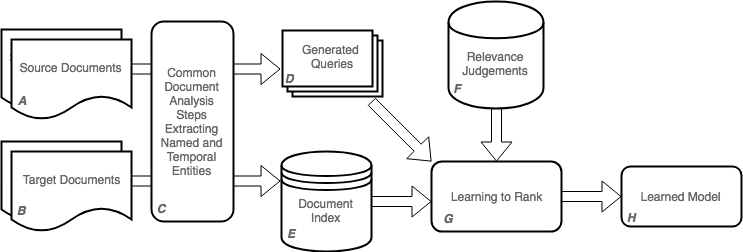
\includegraphics[scale=0.5]{5yp.png}
\end{center}
\caption{\label{fig:approach} The Stages Involved in Producing A Learned Model \remove{label the components in this diagram, refer to in 3.2}}
\end{figure*}

Having given an overview of the method we use in this paper we now give a more concrete explanation of our steps. First we describe the document analysis process used for indexing and query production.

\section{Document Analysis} \label{sec:components}
In this section we describe the components that we extract from documents in order to formulate queries, including our use of named and temporal entities.
These are analysis steps which are common to both source and target documents, however the former produces queries and the latter produces an index of documents for retrieval. This distinction is shown in Figure~\ref{fig:approach}.

The reason for this common analysis is so that terms in queries and indexed documents match during querying. So, if we wish to use some artefact to form a subquery we must ensure the same analysis has taken place on all target documents.
 
We now describe the individual components we extract from documents.

\begin{table*}[t]
\centering
\begin{tabular}{|p{8cm} | p{5cm}|}
\hline
Document Text & Example Complex Query  \\ \hline
\textbf{Dukakis Loses Appeal Challenging Federal Authority Over National
Guard}

   A federal appeals court has rejected \textbf{Democratic} presidential candidate \textbf{Michael Dukakis'} attempt to use his power as governor to block a \textbf{Massachusetts} National Guard training mission in \textbf{Central America}.
   The \textbf{1st U.S. Circuit Court of Appeals} issued a one-sentence order \textbf{Tuesday} affirming a May 6 decision by \textbf{U.S. District} Judge \textbf{Robert Keeton}, who upheld federal supremacy over the National Guard.
   ``Having examined the briefs of the parties ... and having had the benefit of oral argument, we affirm the judgement on the basis stated in the district court's well-reasoned opinion,'' the appeals court said.
   \textbf{Dukakis} sued in January to block the assignment of 13 public relations specialists in the \textbf{Massachusetts} Guard to \textbf{Honduras} and \textbf{Panama} for two weeks in \textbf{May} because of his opposition to \textbf{Reagan} administration policies in the region.
   In his presidential campaign, \textbf{Dukakis} has denounced the administration for its ``failed and illegal'' policy of supporting \textbf{Nicaraguan} rebels, and he said sending Guard troops to the region was an attempt to intimidate \textbf{Nicaragua}.
   \textbf{Dukakis}, who was campaigning \textbf{Tuesday} in \textbf{California} and \textbf{Colorado}, had no immediate comment on the appellate decision. A press aide, \textbf{Steven Crawford}, said the governor was disappointed that the court chose not to uphold the ``important principle'' of state authority. ...
&
\#\textit{sample}\{ Michael Dukakis, Robert Keeton, federal, court, ... \}

\phantom{blah}

\#\textit{persons}\{ Michael Dukakis, Robert Keeton, Dukakis, Reagan, Steven Crawford \}

\phantom{blah}

\#\textit{locations}\{ Massachusetts, Central America, U.S., Massachusetts, Honduras, Panama, California, Colorado\} 

\phantom{blah}

\#\textit{organisations}\{ 1st U.S. Circuit Court of Appeals, National Guard\}

\phantom{blah}

\#\textit{times}\{ May, Tuesday\}

\phantom{blah}

\#\textit{median focus time}\{ 01/01/1988 \}

\phantom{blah}

\#\textit{vf focus time}\{ 01/01/1988 \} 

\phantom{blah}

\#\textit{other terms}\{ federal, appeals, court, reject, presidential, candidate, attempt, power, governor, block, training, ...\} 

\\ \hline
\end{tabular}
\caption{An Example Representation of a Complex Query Created From a Document}
\label{table:complexquery}
\end{table*}

\subsection{Named Entities}
We have seen from Section~\ref{sec:background} that named entities are a valuable artefact to extract from documents for query formulation. Encouraged by the results from~\cite{DissertationKelvinFowler} we continue to use named entities in queries

% In this paper we will only consider named entities referring to persons, locations or organisations. 

In this project named entities are extracted using the Stanford NLP NE Recogniser~\cite{manning2014stanford}. We extract 3 types of named entities: people, locations and organisations. We are careful to maintain multi word named entities to avoid loss of information addressing \textbf{Limitation 1}. For example, there are likely many mentions of ``Hillary'' and ``Clinton'', but far fewer mentions of ``Hillary Clinton''.

There may be many different named entities in a document and some may be mentioned more than others.
As such we use TF-IDF to calculate which terms in our document are most important.
% Show proportion of top-k terms which are named entities?

\subsection{Temporal Entities}
\remove{what do you do in one sentence, what do you do abstractly, then give a concrete example using an example document}
\remove{The description here of the analysis needs to be much clearer, introduce nice notation for median and vf focus times}
\textbf{Limitation 3} specifically highlights the lack of use of temporal entities in our previous approaches to this task and~\cite{alonso2011temporal,jatowt2013estimating} show that inclusion of temporal entities is beneficial in other tasks.
In order to include any sort of temporal information in our queries we must first retrieve this information from the source documents.

Temporal entities were resolved using the Heideltime temporal tagger~\cite{strotgen2010heideltime}. This allows us to identify temporal entities in text such as ``last Thursday'' and resolve this reference the specific date in question. In order to do this resolution it is necessary to know the document creation date. 
Examples can be seen in Table~\ref{table:focustimes}.

% math mode version
From a given document $D_{text}$ which is a bag of words we can extract and resolve all of the temporal entities. This gives us a temporal representation of this document, the set of all times in the document $D_{temp}$.

% we dont expect just using these plain temporal entities to be good, why?
It is a reasonable assumption that these specific times are not of great use in and of themselves, since they are so numerous and so granular that matching on them will not produce any interesting behaviour (we confirm this with results in Section~\ref{sec:results}). As such it seems that it would be helpful to perform some analysis on the temporal entities that occur in a document.

% explain the focus time alternative
We have opted for two approaches of calculating the focus time of a given document which contains temporal entities.

The first is a calculation of the median of all times mentioned in the document. In order to calculate the median focus time all temporal references in a document are converted to their epoch offset equivalent (milliseconds from Jan. 1st 1970).
This collection was then sorted and the median date was taken to be the focus time.
This median time was then used to create 3 terms, a focus day, month and year.
This allows for different granularities of matching.
Two document which matches exactly on the median focus day are likely to be referring to very similar temporal entities within their text. The relationship will be weaker for month and year granularities.

% Be inspired by heideltime paper for mathsy way to reperesent focus times.

% The first, median focus time $FT_{med}$, simply sorts the temporal references in a document and takes the median, assuming this to be some indication of the time which a document refers to.
% $FT_{med} = median()$
    
%why vf focus time?
The second uses the notion of value frequency in order to calculate a focus time. In \cite{strotgen2012identification} value frequency is used as an indicator of the importance of temporal entities in a document, inspiring us to also use this measure.

We consider three sets of temporal entities $Y, M, D$ 

Y mentions years and contains every temporal entity which mentions a year.
2010, may, and today all fit into this category as they all refer to a specific year. Last century does not fit in to this category.

M and D are defined in similar ways.

For all entities in Y, we count the occurrences of the various years mentioned and select this to be the vf focus year.

For all entities in M, we count the occurrences of the various months mentioned and select this to be the vf focus year. These are specific months in years, i.e there will be a count for 03/89 and 03/88 as these are not the same month and documents could refer to both.

Same story for D.


% We want this to be a table which has times in it, then shows how these times become median focus times and vf focus times

\begin{table}[t] 
\centering
\begin{tabular}{|c|c|}
\hline
Temporal Entity 	& Resolution 					\\ \hline
Last Thursday 		& 14/04/1988   \\ 
Today				& 18/04/1988 \\ 
1988 				& 1988  \\ 
January 			& 01/1988   \\ 
Sunday 				& 13/04/1988   \\ 
Tonight				& 18/04/1988 \\ 
This Year 			& 1988   \\ \hline \hline
Median Date			& \textbf{CALCULATE} \\
Vf Year				& 1988	\\
Vf Month			& 04/1988	\\	
Vf Day				& 18/04/1988	\\ \hline
\end{tabular}
\caption{Examples of Resolved Temporal Entities and Subsequent Calculated Focus Times For A Document Created on Monday 18/04/1988}
\label{table:focustimes}
\end{table}

 
\subsection{Additional Terms}
In addition to named and temporal entities there are many other terms in a document. These provide valuable context for the reader, and as we have seen from our example in Table~\ref{table:example} would generally be necessary in a query to produce high quality results.

After identifying named entities and temporal entities we can simply identify these other terms as those which are left over. We can tag these as belonging to the ``other'' set.

It is worth noting that not all of these terms will be valuable to us and so we use Tf-Idf in order to identify which terms are most important from a given document.

Having explained our steps for the analysis of documents for the creation of queries and indexing, we now move on to explain our use of learning to rank in combination with complex queries.

\section{Learning with Complex Queries} \label{sec:l2r}
This section gives details on our method of using learning to rank to implicitly learn the importance of sections of queries formed from documents.
The queries we formulate contain many distinct parts.
Unfortunately we do not know which parts of the query are most important for our task. Unlike Lee et al~\cite{GeneratingQueriesLee12} we wish to calculate this importance within the context of our specific task and datasets.

Learning to rank uses relevance judgements and so, we can know that the learner will be trying to optimize retrieval performance rather than any other metric. If we were to use pre-calculated features we could be inferring relationships which are not true. Using learning to rank prevents any incorrect assumptions being factored into the model.

We specifically wish to use learning to rank as a method for understanding the implicit importance our subqueries and so we must define features which represent this.
This is not possible using the standard bag of words model and so we reformulate our query into specific sections. This accomplished using complex query operators.

Complex query operators can be found in the Indri Complex Query language~\cite{strohman2005indri} and are present in Terrier~\cite{macdonald2012puppy}. They allow the formulation of queries with additional rules such as defining synonyms or adding term proximity limitations.
We use the tagging features of the Indri Complex Query language which allow us to label individual sections of queries with different tags.
For example, we separate and label person named entities and organisation named entities and have tags for our various focus time calculations.

With these subqueries we can define features which are only calculated with respect to individual subqueries. Applying this learned model on subsequent queries is in effect applying a weighting scheme to the individual subqueries.

Table~\ref{table:features} defines all of the features used in our learning to rank approach.

\begin{table*}[t] 
\centering
\begin{tabular}{|p{2cm}|p{4cm}|p{6cm}|}
\hline
Feature Ref   & Feature Name 		& Description  \\ \hline
$DPH_{sample}$ & Sample Terms DPH 	& DPH Score for Terms used in Sample Query \\ \hline
$TF_{person}$ &Person TF 		& TF Score for Person Named Entities \\
$TF_{loc}$&Location TF 		
& TF Score for Location Named Entities 		\\ 
$TF_{org}$&Organisation TF 	
& TF Score for Organisation Named Entities  \\
\hline
$BM_{time} $&Time Terms Constant 
& Constant WM Matching on Temporal Terms    \\
\hline
$Bin_{VFyear}$ & Vf Focus Year 		
& Binary Matching on most frequently mentioned year. \\
$Bin_{VFmonth}$ & Vf Focus Month 		
&Binary Matching on most frequently mentioned month (YY-MM). \\
$Bin_{VFday}$ & Vf Focus Day 		
& Binary Matching on most frequently mentioned day (YY-MM-DD).\\
\hline
$Bin_{medyear} $& Median Focus Year 	
& Binary Matching on Median Calculated Focus Year 		  \\ 
$pBiL_{medmonth} $& Median Focus Month 	
&Matches of Same Adjacent Median Year, Month, Day Focus Terms (pBiL~\cite{pbil}) \\ 
$pBiL_{medday} $& Median Focus Day 	
& Matches of Same Adjacent Median Year, Month, Day Focus Terms (pBiL~\cite{pbil}) \\ \hline
\end{tabular}
\caption{Features Used in this Paper}
\label{table:features}
\end{table*}

\subsection{Sampling}
\remove{need a better explanation of this sampling step and how the recall of the pool effect retrieval, whens and hows}
Since learning to rank is used to re-rank the top $k$ documents based on a certain set of features, it is important that this set of documents being re-ranked contains the highest possible number of relevant documents.
We aim to maximise recall at the initial stage of learning to rank so that upon reranking based on features we can promote as many relevant documents as possible.

Recall is a measure of how many of the relevant documents were retrieved.
It is possible to achieve 100\% recall \remove{is this good} simply by retrieving all documents, however the calculation of feature scores across this amount of documents would take far too long for our needs. Why? Because we want fast retrieval~\cite{NEEDED} and people are only willing to wait so long on queries.

We now move on to describe our experimental set-up and experiments conducted using the above explained method.

\section{Experimental Set-up} \label{sec:setup}
% introduction
This section will describe the steps taken to evaluate our system. We describe the test collections we use as well as the learning to rank configuration.

% Research Questions and Explanation
\subsection{Research Questions}
We begin by defining formally the research questions which we seek to answer through this evaluation.
\begin{enumerate}[label=\textbf{RQ.\arabic*}]
\item How can we maximise recall at the sampling step of retrieval to achieve the best results using learning to rank?

\item What information in source documents is most important for the retrieval of public domain documents containing information in the source document?

\item Can we combine these results to create a comprehensive retrieval model in order to retrieve public domain documents helpful to the sensitivity review task?
\end{enumerate}

\subsection{Test Collections}
% explain why last years test collection isn't suitable
In the previous L4 Project~\cite{DissertationKelvinFowler}, a small test collection was manually created. The topics were queries formed from 20 government documents, each of which had an associated 20 relevant public domain news articles. 
Because our approach in this research involves the use of learning to rank, we require a much larger collection of relevance judgements~\cite{NEEDED}. 
It was not feasible create more manual relevance judgements as this would have been a very time consuming task.
Thus it was necessary to produce a test collection by some other means.

% explain why we can use the proxy approach
\remove{need some stronger evidence, analysis with numbers, give an example}

Having analysed the government documents collection of source documents it became clear that these documents generally followed a similar structure of reporting events from the viewpoint of various embassies. These reports exist to inform a reader about events happening at specific times, involving people, organisations and locations.

Now, news articles are very similar in nature to the government documents in our source collection, as they also seek to report on events, the difference being that the content of a news articles is necessarily already in the public domain.
This similarity suggests that it may be possible to use news articles as representative source documents for the generation of queries.

Unfortunately, we did not have access to relevance judgements which defined news document as being relevant to one another.
Instead we chose to use the implicit relevance of documents to one another which are relevant for a common topic.

Given an existing TREC ad-hoc topic there exists a set of relevant public domain news articles. If two articles are relevant for the same topic, it suggests there is some information overlap in these documents.

Thus we made the assumption that if documents were relevant for the same topic then they were relevant to each other in our public domain comparison task.

% explain in words how we make proxy

Since we are only using AP88 \remove{this is not state before hand} as our test collection relevance judgements concerning any other documents were removed and ignored.

If we take one of these proxy source documents S, the list of relevant target documents will include the original target document S. S must be removed from the relevance judgements.
A document can not be relevant for the query generated from itself. This caveat allowed us to avoid any additional complex indexing strategies.

The method described below for generating a test collection from existing topics and query relevance judgements are inspired by a method described by Lee et al~\cite{GeneratingQueriesLee12} for choosing text segments from documents to generate queries from. Lee et al ensure that the text segments align with the TREC topic descriptions, meaning the relevance judgements can be used, but we don't do that, \remove{so that's probably an issue.} 

\remove{use an algorithm format here, will look better}

We have a set $T_C$ of public domain documents.

Let us take 1 query from the topic set, $ q \in Q $.

There is a set of documents with judgements for $q, J_q \subseteq T_C$.

There is set of documents which are relevant $R_q \subseteq J_q$.

Let this $R_q$ become our new $S_C$, the collection of source documents from which we form queries.

If we form a query $ Q_d $ from a document $ d $ in in $ S_C $ the we assume judgements of $ J_q \setminus d$ apply. 

\paragraph{explain formally how we make proxy}
% Explain the algorithm, write on paper to get right first.
\begin{algorithm}
\SetAlgoLined
\KwResult{Proxy Test Collection}
 $T_C$, the set of target public domain documents
 
 $ Q $, the set of TREC topics
 
 $S_C = \emptyset$, the set of source documents
 
 $Qrels = \emptyset $, the set of relevance judgements for $S_C$
 
 \For{each query $q$ in topic set $Q$}{
 
 get documents with judgements for $q, J_q \subseteq T_C$
 
 get set of documents which are relevant $R_q \subseteq J_q$
 
 \For{each doc $d$ in relevant docs $R_q$}{
 	add judgements of $J_q \setminus d$ to judgements $J$
 }
 
 add $R_q$ to $S_C$, 
 
 If we form a query $ Q_d $ from a document $ d $ in in $ S_C $ the we assume judgements of $ J_q \setminus d$ apply
 }
 \caption{Generating a Proxy Test Collection From Existing Relevance Judgements}
\end{algorithm}

\paragraph{statistics}
We use several different collection of documents and queries in this work.
Our proxy test collection is generated 1988 Associated Press (AP) news articles found in TIPSTER disk 2.
TREC-1 ad hoc topics 51-100 have relevance judgements for  TIPSTER disks 1\&2. We ignore all relevance judgements for documents outside of the 1988 AP Collection.

The 1988 AP collection contains 79919 documents.

Our method of producing source documents from this collection provided us with 2742 source documents.
When creating a query from one of these source documents, that document is remove from the target collection and so retrieval using this collection only ever takes place with 79918 documents.

In addition to this proxy test collection we have a small collection of government documents with relevance judgements for public domain documents.

This set of public domain documents are Reuters in 2008 and there are 101253 of them.

We create queries from 20 government documents however we index 1018 documents for the purpose of calculating Tf-Idf scores for term importance.

\begin{center}
\begin{table}[H]
\centering
\begin{tabular}{|c|c|}
\hline
Collection	 	& Documents 		\\ \hline
AP88			& 79919				\\
Reuters 2008	& 101253			\\
Govt. Source 	& 2742				\\
Govt. Source w/ Judgements & 20	\\ \hline

\end{tabular}
\caption{Test Collection Statistics}
\label{table:statistics}
\end{table}
\end{center}

\subsection{Verification Using Government Document Test Collection}
In order to verify that our approach of using the proxy test we also use a small test collection which was created last year using documents which are representative of those considered sensitive. These are government documents. \remove{GIVE DETAILS}

\subsection{Learning to Rank}
\paragraph{Explain Learning to rank approach}
Our learning to rank model is the Jforests implementation of LambdaMART  which uses multiple additive regression trees and is a combination of pointwise and listwise learning to rank approaches.~\cite{NEEDED}

\remove{give example of regression tree}

% explain partitioning of data - whens and hows of learning to rank may be able to help
In order to prevent over-fitting to training data during learning to rank we partitioned our test collection into training, validation and test sets.
This was done with a 60/20/20 ratio.
The splitting was performed by partitioning the initial topic set rather than the proxy test collection \remove{WHY?}.

% \subsection{What are we looking for}
% Likely, our strongest feature is the one which increases MAP the most, what if none of them increase MAP! This will be the feature sends relevant documents in the k sized sample towards the top. (map)
% We may have some much weaker features which alter the rankings of the top few documents. These are also important as they will directly effect the results that are looked at first during manual inspection. (p.5 and mrr).


\section{Experimental Results} \label{sec:results}
In this section we address \textbf{RQ1} and \textbf{RQ2} which are evaluated on the AP88 collection with proxy relevance judgements.

\subsection{RQ1 - Recall During Sampling Step} \label{sec:RQ1}
% Introduce
This section covers \textbf{RQ1} by investigating how we can build a sample query which gives us high recall. We need a high recall sample of documents for re-ranking based on various features.
Additionally, we are concerned with the time it takes to perform this initial query step, as users are only willing to wait for search results for so long~\cite{brutlag2009speed}.

% Explain what experiments we are doing
\remove{use present tense}
Using the system of subqueries discussed in Section~\ref{sec:l2r}, we now have complete control over the terms which will be used to obtain this sample pool of documents for reranking. We will call this subquery the \textbf{sample subquery}.
The experiments in this section deal with altering the contents of this sample subquery to obtain the best recall scores possible while maintaining efficiency.
We alter the number of terms in the sample subquery and we also use TF-IDF weights on each term.
The number of terms is altered by taking the top k terms when ordered by TF-IDF score calculated over the AP88 collection.
In addition, we alter the retrieval model used when obtaining this sample to ensure we have chosen the model which gives the highest recall.

% Expectations
We expect that having more terms in the sample subquery will improve recall scores, however will slow down results. We expect that query terms being weighted with TF-IDF scores will improve recall further.

% We expect that just using other terms would be bad
% Just using named entities would be bad -- for recall.

% Experiment Pre-amble
We report recall scores averaged over 1371 source documents in the training partition of the proxy test collection. Recall is calculated using the associated proxy relevance judgements.
We also report the average time taken per query.
In all of the experiments in this section we return 1000 documents per query.

% Retrieval Model Experiment
First, in Table~\ref{table:recallmodel} we report the recall scores of using the top 100 terms weighted with TF-IDF using 5 different common retrieval models.
\begin{table}[H]
\centering
\begin{tabular}{|c|c|}
\hline
Model	 		& Recall 				\\ \hline
DPH 			& \textbf{0.6928} 		\\
TF-IDF 			& 0.6853 				\\
TF 				& 0.6627 				\\
PL2 			& 0.6324 				\\
BM25 			& 0.5758 				\\ \hline
\end{tabular}
\caption{Recall with Different Retrieval Models, Query Size 100, Terms Weighted with Tf-Idf}
\label{table:recallmodel}
\end{table}

We see from Table~\ref{table:recallmodel} that DPH~\cite{NEEDED} provides the highest recall score of the 5 retrieval models we test. Given this result, we use DPH as the retrieval model for the following experiments which alter the terms used in the sample subquery.

% Query Size Unweighted
We now investigate which terms we should use in our sample subquery in order to achieve maximum recall within a reasonable time. We score each term in the source document with its TF-IDF score with respect to the entire collection and sort these from highest to lowest. We take the top $k$ terms under this scoring system and report the results in Table~\ref{table:sample_size_uw}.
We also use \textit{all} terms in a subquery, this means we do not cut off the ordered terms at any $k$. Across 1371 queries, when using all terms,  the average query length was 221, the smallest query was 52 terms and the largest was 540.
We see that using the top 100 terms gives us the highest recall score when the terms are added to the sample subquery with equal weights. As expected, the subquery with the smallest size performs the fastest on average.

\begin{center}
\begin{table}[H]
\centering
\resizebox{\columnwidth}{!}{%
\begin{tabular}{|l|c|c|}
\hline
Size	 			& Recall 		& Mean Query Processing Time (s) \\ \hline
All 				& 0.6082 		& 0.4400    	        \\ 
250					& 0.6163		& 0.3792			    \\ 
100 				& \textbf{0.6534} 		& 0.1216    	\\ 
50 					& 0.6480 		& 0.0557    	        \\ 
25 					& 0.6243 		& 0.0481    	        \\ 
10 					& 0.5708 		& \textbf{0.0357}    	 \\ \hline
\end{tabular}%
}
\caption{Recall and Average Processing Time with Different Sample Subquery Sizes, Unweighted Queries w/ DPH. Results over 1371 queries.}
\label{table:sample_size_uw}
\end{table}
\end{center}

When using DPH, we also have the ability to weight the terms in our sample subquery with a given weight. We can assign to each term its calculated TF-IDF score.

% Query Size Weighted
We repeat the previous experiment with these per term TF-IDF weights applied and report the results in Table~\ref{table:sample_size_w}.

\begin{center}
\begin{table}[H]
\centering
\resizebox{\columnwidth}{!}{%
\begin{tabular}{|l|c|c|}
\hline
Size	 		& Recall 	& Mean Query Processing Time (s)	\\ \hline
All 			& 0.6904 	& 0.4856    	          	\\ 
250 			& \textbf{0.6908}	& 0.4277					\\ 
100 			& 0.6824 	& 0.1203   	          	   	\\ 
50 				& 0.6619 	& 0.0673    	          	\\ 
25 				& 0.6324 	& 0.0598    	     	   	\\
10 				& 0.5750 	& \textbf{0.0273}    	    \\ \hline
\end{tabular}%
}
\caption{Recall with Different Sampling Sizes, Weighted Queries w/ DPH. Results over 1371 queries.}
\label{table:sample_size_w}
\end{table}
\end{center}

We see from Table~\ref{table:sample_size_w}, that this markedly improves the results of various sizes of sample subquery, with the 250 term subquery performing best in terms of recall. Again, as expected the smallest query is performed fastest on average.

We notice, however that although the 100 term sample subquery is produces a slightly worst recall than \textit{All} and \textit{250}, it is completed in less that half of the average time. This is important to us, as sampling is only the first step in learning to rank.
The calculation of subsequent features can be a time intensive task~\cite{NEEDED} and so a fast sampling stage is desirable.

% Conclusion on this research question.
The conclusions we draw from the data reported with regards to \textbf{RQ2} is that more terms in the sample subquery seems to produce improved recall scores, up to around 250 terms. We also see significant increases in recall by weighting terms in our sample subquery using TF-IDF scores. Although this 250 term weighted query produces the highest recall out of all of our experiments, it takes more the double the average time to execute compared to a 100 term query.
For this reason we conclude that a 100 term weighted sample subquery issued under DPH produces sufficient recall in an acceptable time for the sample section of learning to rank.

% Link to Next Section
We now move on to report our findings regarding feature importance during the reranking of this sample, addressing \textbf{RQ2}.

\subsection{RQ2 - Feature Importance} \label{sec:RQ2}
% What do we want to find out
We now investigate feature importance, in response to \textbf{RQ2}. In order to gain a clear understanding of which features are important we perform several experiments using learning to rank with different combinations of the features defined in Table~\ref{table:features}.
In addition we analyse the distributions of our various features in order to predict what performance we might expect.

% what are the experiments
For all of these experiments, we fix the sampling subquery to be the top 100 terms based on their TF-IDF score. These terms are weighted with this TF-IDF score and the retrieval model for the sample subquery is DPH. This is based on the findings from \textbf{RQ1}, which suggest that this approach is effective and efficient.

Our experiments will examine the effect on precision that reranking based on these features has. Learning to rank will be training on the set of training source documents from the generated proxy AP88 source collection. We also use a validation set of source documents from this collection to prevent overfitting.
The results reported are here are the retrieval performance scores from applying the learned model to retrieval on the test partition of the AP88 source document collection.

We report all of these results in Table~\ref{table:rq2_results}.

% what are our expectations?
% Named Entities
We expect that named entities will help.
Why? because look at the distribution graphs.
Relevant documents are more likely to have high tf scores when matching on people, places and organisations.

% Temporal Entities
We do not expect that explicit matching on individual temporal entities will be an effective feature in learning to rank. For any given documents there are going to be many temporal entities. These will be far too varied and numerous for explicit matching to improve results.

% Focus times
Our focus time calculations on the other hand, could offer some improvement when used as a feature. It is likely that if two documents focus on the same time then they will be relevant to each other.
Median focus time will be helpful in identifying documents which mention distinct dates as the median will lie in the centre.
Value frequency calculated focus time will be helpful for boosting the scores of documents which make reference to many of the same dates as the source document.
Our training collection only consists of documents from 1988 and so there may be an issue involving the focus date being skewed towards this date.
We can see this from ... there is going to be excessive amounts in 1988 etc.

All documents in our test collection for training are likely to have a similar focus year, since they are all documents from 1988. This means that our $VF_{year}$ feature is likely perform poorly in comparison to a collection which references many different years.

\paragraph{expectations backed up by distribution graphs}
\remove{i had been looking at the wrong things}
\remove{reference the method you use to produce these graphs}
\begin{figure}[H]
\begin{center}
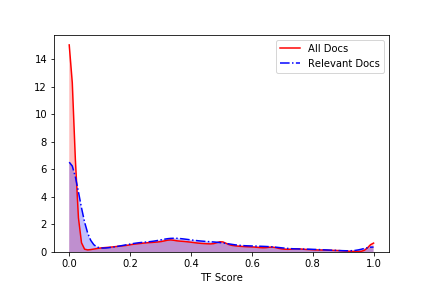
\includegraphics[scale=0.5]{persons.png}
\end{center}
\caption{\label{fig:distribution} Feature Distribution over All Documents vs Relevant Documents}
\end{figure}
\begin{figure}[H]
\begin{center}
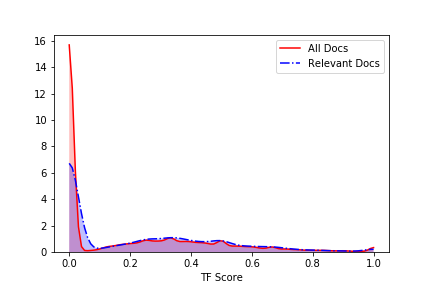
\includegraphics[scale=0.5]{orgs.png}
\end{center}
\caption{\label{fig:distribution} Feature Distribution over All Documents vs Relevant Documents}
\end{figure}
\begin{figure}[H]
\begin{center}
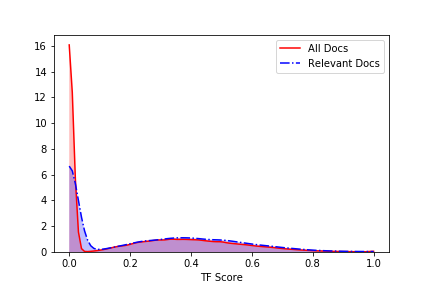
\includegraphics[scale=0.5]{locs.png}
\end{center}
\caption{\label{fig:distribution} Feature Distribution over All Documents vs Relevant Documents}
\end{figure}

% Define a baseline
Our baseline for the following experiments will be the performance of the sample subquery which is obtained before re-ranking. This allows us to see the impact on performance the re-ranking based on different features has.
In all of the following experiments, the recall reported does not change between the reported baseline and the re-ranked results, indicating clearly that the set of retrieved documents is the same, however the specific ranking order has been altered due to the features.

These baseline results can be seen in the first row of Table~\ref{table:rq2_results}, denoted by an empty feature set, $\emptyset$.

We can use the sample subquery to define a feature, $DPH_{sample}$, which is the score of a given document calculated via DPH on the sample subquery.

% Named Entity Features
The results of using named entities based features are not promising on the proxy test collection.
Rather than improve precision, the results are actually degraded. \remove{is this significant}.
What exactly is the TF feature on the different types of named entities.
We take an individual type of named entity and for this subset of terms we calculate the TF (or other measure) score.
Our intuition is that documents with a higher tf score for the given subquery are more likely to be relevant to the source document.

We can see an example of a proxy source document which exhibits this relationship in Figure~\ref{}

What we see is that relevant documents are more likely to have a high tf score with respect to the person subquery.
% include image of the really nice distribution graph


What is unfortunate is that this distribution which suggest these features would be successful does not carry over when we plot the same distribution over all of the training documents as can be seen in Figure~\ref{}. Both Figures x and y are only plotted on the persons named entity subquery, however a similar picture can be seen for organisations and locations.

% Temporal Entities
We expect that binary matching on individual temporal terms will not be a helpful feature.

% Focus Times
We suspect that to make use out of temporal entities we must 

\begin{center}
\begin{table}[H]
\centering
\resizebox{\columnwidth}{!}{%
\begin{tabular}{|l|ccc|}
\hline
Feature Set	 			& MAP 		& MRR  			& P@5 		\\ \hline
$\emptyset$		   			
& \textbf{0.2013} 	& \textbf{0.6229}    	& \textbf{0.4338}  	\\ \hline
$DPH_{sample}$   		
& 0.1898 	& 0.6048	    & 0.4131	\\ \hline
$DPH_{sample}, TF_{person}$				
& 0.1840    & 0.6025    	& 0.4044    \\ 
$DPH_{sample}, TF_{org}$		
& 0.1855	& 0.6063 		& 0.4015	\\
$DPH_{sample}, TF_{loc}$ 			
& 0.1859 	& 0.6005    	& 0.4020 	\\ 
$DPH_{sample},TF_{person},TF_{org}$ 	
& 0.1784 	& 0.5989    	& 0.4041	\\ 
$DPH_{sample},TF_{person},TF_{loc}$ 	
& 0.1634 	& 0.5939		& 0.3974	\\
$DPH_{sample},TF_{loc},TF_{org}$ 	
& 0.1843  	& 0.6139   	 	& 0.4023	\\ 
$DPH_{sample}, TF_{person}, TF_{org},TF_{loc} $ 				
& 0.1553 		  & 0.6004   	 	& 0.3948	      \\
$DPH_{sample}, TFIDF_{person}, TFIDF_{org},TFIDF_{loc} $ 				
& 0.1842 		  & 0.6087   	 	& 0.4105	      \\ \hline
$ DPH_{sample}, Bin_{time} $	
& 0.1885 		  & 0.6213   	 	& 0.4134	      \\ \hline
$DPH_{sample},Bin_{VFyear},Bin_{VFmonth},Bin_{VFday}  $ 	
& 0.1878 		  & 0.6143   	 	& 	0.4140       \\
$ DPH_{sample},Bin_{VFmonth},Bin_{VFday} $ 
& 0.1827 		  &  0.6123  	 	& 0.4096	      \\ 
$ DPH_{sample},Bin_{VFmonth} $ 	
& 0.1886 		  &  0.6199  	 	& 0.4125	      \\ \hline
$ DPH_{sample}, Bin_{MEDyear}, pBiL_{MEDmonth}, pBiL_{MEDday} $ 	
& 0.1763 		  & 0.5929   	 	& 0.3956	      \\ \hline
$ DPH_{sample},TF_{person}, TF_{org},TF_{loc},Bin_{VFmonth}  $	
& 0.1780 		  & 0.5995   	 	& 0.3962	      \\ \hline
\end{tabular}%
}
\caption{Learning to Rank with Various Feature Combinations, Evaluated on Proxy Test Collection formed from AP88}
\label{table:rq2_results}
\end{table}
\end{center}

\remove{bold best results}

\remove{can we do signifigance testing}

\paragraph{comparison to expectations -- likely lower}
Our results do not show any increase versus the baseline results, which indicates that reranking based on the features is not helpful in this instance.
In contrast to our feature distribution graphs, this is somewhat surprising. We expected that with more relevant documents obtaining higher feature scores, especially for named entity features, the learned model would reflect this.
It may be the case that the features introduce too much noise and the distinction in score between relevant and non-relevant docs is too great.

\paragraph{failure analysis - why didn't it work}
We can inspect some individual examples of queries which performed better with the use of these features.
Specifically a good example is ... \remove{give an example of a query which performed well.}
It didn't work because the feature distributions don't show any correlation over the full collection.


% Failure Analysis - Look at an Example Document
% Use precision at 5 for these tests.
% Want to know which document came in this top 5?

\section{Evaluation on Government Documents} \label{sec:RQ3}
In this section we show our results when evaluating our methods on a test collection composed of government documents with relevant public domain documents.

% What Sampling step and why?
Again, we continue to use the 100 Weighted Terms sampling step.

% What features and why?
With no clear combination of features that performs exceedingly well we repeat some of the above experiments.

%report MAP from last year
In the L4 Project~\cite{DissertationKelvinFowler} we reported the results shown in Table~\ref{table:lastyears}. Both queries in Table~\ref{table:lastyears} are simple bag of words queries. The all terms query was created by using all terms in the source document.
The named entities query was created by only using the people, location and organisation named entities as a bag of words query.
We reported P.4 as the produced UI showed 4 documents in the initial search results.
Our conclusion in the L4 Project was that named entities were clearly an important factor in this retrieval task, because the although the results were degraded when not using other terms, this was only by a small amount. Using only the named entities as a query was also much more efficient.
The performance of the bag of words named entity query in the L4 Project was a strong contributor to the selection of named entities to form subqueries for features in learning to rank. %More on this later.

\begin{table}[h]
\centering
\begin{tabular}{l|ccc}
Query Type 		& MAP 		& MRR 		& P.4 		\\ \hline
All Terms 		& 0.4554 	& 0.8500  	& 0.6750   	\\
Named Entities 	& 0.3979 	& 0.7526 	& 0.5875    
\end{tabular}
\caption{Results of Evaluation from L4 Project}
\label{table:lastyears}
\end{table}

We cannot use the results from Table~\ref{table:lastyears} as a baseline when performing the evaluation in this section using our new techniques. 
This is because we use a subset of the source and target collection due to time constraints. The test collection statistics are reported in Table~\cite{NEEDED}.
As such, we report the results of using bag of words queries on these test collections in Table~\ref{table:rq3baseline}. Our use of named entities has, however, changed slightly as we now maintain multi word named entities, as discussed in Section~\ref{sec:components}.

\begin{table}[h]
\centering
\begin{tabular}{l|cccc}
Query Type 		& MAP 		& MRR 		& P.5 		& Recall	\\ \hline
All Terms 		& 0.4337 	& 0.7988  	& 0.5700	& 0.8299   	\\
Named Entities 	& 0.3863 	& 0.7052 	& 0.4600    & 0.9746
\end{tabular}
\caption{The same evaluation, but on this years data}
\label{table:rq3baseline}
\end{table}

We define the results of Table~\ref{table:rq3baseline} as a baseline because they represent our previous understanding of the task.

Our experiments will follow a similar structure to those in Section~\ref{sec:RQ2}, reporting the results of the sample subquery followed by the changes observed when reranking based on various features during learning to rank. We use the same learned models from the AP88 data as in Section~\ref{sec:rq2}. Again, this is because we do not have sufficient training data in the government document test collection.

% what do we expect
From analysing the result of Section~\ref{sec:rq2} we do not expect to see any significant increase in results when using our new features.
We are unsure how the sample subquery will perform, as it may prove to be a better alternative bag of words query than those investigated in the L4 Project.

In Table~\ref{wikileaks_results} we report the results of using our learned models on the government test collection. Again the first row represents the performance of the sample subquery alone with no feature based reranking.

% results on wikileaks collection
Recall does not change across the following results, it is always 1.
\begin{center}
\begin{table}[H]
\centering
\resizebox{\columnwidth}{!}{%
\begin{tabular}{l|ccc}
\hline
Feature Set	 			 & MAP 		& MRR  		& P@5  		\\ \hline
None		   			 & 0.5842 	& 0.8375    & 0.6500  	\\ \hline \hline
Sample DPH		   		 & 0.5547	& 0.8667    & 0.6100  	\\ 
Sample DPH, TF NE		 & 0.5013	& 0.8083    & 0.5700  	\\ 
Sample DPH, VF Month     & 0.5541	& 0.8417    & 0.6300    \\ 
Samps DPH,TF NE,VF Month & 0.5339	& 0.7517	& 0.6100	\\ 
\end{tabular}%
}
\caption{Learning to Rank with Various Feature Combinations on Real Government Documents Collection}
\label{wikileaks_results}
\end{table}
\end{center}

Inspecting Table~\ref{wikileaks_results} we see that, in comparison to the bag of words queries tested in Table~\ref{table:rq3baseline}, there is an increase over all reported measures.
We are specifically interested in the performance of the P@5 measure. This is the precision of the top 5 documents returned, which are likely the first that manual reviewer would examine.
Comparing the all terms bag of words query with the sample subquery we find that neither is statistically significant when using the two tailed students t-test with a p-value of 0.05.

What about MAP, does that increase significantly:
For the sample subquery map does increase significantly when using the two tailed students t-test with a p-value of 0.05 vs the named entity bag of words query.
This means that we at the very least have a new way to get results.

\textbf{per query failure analysis}
Lets first do per query improvements over the 20 queries.
No queries improved when using Sample DPH and TF NE as features.


\remove{tokyo query has very nice distributions for org and loc, do we have any results that show this improved over baseline}
We can analyse individual queries to gain a better understanding of why we did not achieve an increase in performance when using the features.

In order to answer this question we must consider what is a baseline for good performance. We assume a baseline as being the retrieval scores of simple doing retrieval using a full document as a query on a completely plain index with no additional information in it.

% use of best features
In Section~\ref{sec:RQ2} we evaluated which features we deemed most important for our retrieval task. In this section we show retrieval results when combining these features.
We test this on our existing test collection in addition to our test collection from last year.

\section{Conclusions} \label{sec:conclusion}
\remove{recap aim}
Our aim in this research was discover if learning to rank could be used to improve the performance of retrieving public domain documents from queries generated from source documents.

We found that we can produce a high recall sample of documents by using the top 100 terms from a source document under a TF-IDF weighting scheme.

Of the features we defined none showed any improvement over the baseline of the learning to rank sample subquery. Having examined the data we conclude that our feature selection was poor and distributions graphs extracted from the training data could have predicted this lack of performance for the named entity features.

\paragraph{what did we learn}
We probably should have investigated additional features
We probably should have made use of proximities and other features using the complex query operators.
We probably could have predicted that our features wouldnt work had we run proper analysis on them. - Discovered this too late to do any additional experiments.

We presented an investigation into using learning to rank to effectively learn query formulations when producing queries from government documents. Of the features we defined, none showed improvement over a baseline of using the top 100 terms weighted with tf-idf as a query.
The relationships are not clear enough.


The more features you add, the worse the results get.
Suggests that the features add too much noise to be useful.

% Improvements
More careful feature selection.
First investigation.

% Future Work
In the future we would like to incorporate knowledge base linking into the process in order to flesh queries out with additional details and synonyms for named entities. This could provide an excellent query expansion opportunity.

\vskip8pt \noindent
{\bf Acknowledgements.}
I would like to thank my supervisors, Craig Macdonald and Graham McDonald for their guidance and patience during this project.
\bibliographystyle{abbrv}
\bibliography{bib}

\end{document}

\documentclass{article}
\usepackage[utf8]{inputenc}
\title{L5 Dissertation}
\begin{document}
\url{http://sigir.org/wp-content/uploads/2018/01/p032.pdf}
\end{document}
